\documentclass[a4paper,12pt]{article}
\usepackage[top = 2.5cm, bottom = 2.5cm, left = 2.5cm, right = 2.5cm]{geometry}
% Unfortunately, LaTeX has a hard time interpreting German Umlaute. The following two lines and packages should help. If it doesn't work for you please let me know.
\usepackage[T1]{fontenc}
\usepackage[utf8]{inputenc}
% The following two packages - multirow and booktabs - are needed to create nice looking tables.
\usepackage{multirow} % Multirow is for tables with multiple rows within one cell.
\usepackage{booktabs} % For even nicer tables.
% As we usually want to include some plots (.pdf files) we need a package for that.
\usepackage{graphicx}
\usepackage{tikz}
% The default setting of LaTeX is to indent new paragraphs. This is useful for articles. But not really nice for homework problem sets. The following command sets the indent to 0.
\usepackage[spanish]{babel}
\usepackage{setspace}
\setlength{\parindent}{0in}
% Package to place figures where you want them.
\usepackage{float}
% The fancyhdr package let's us create nice headers.
\usepackage{fancyhdr}
\usepackage{amsmath}
\usepackage{amssymb}
\usepackage{natbib}
\usepackage{apalike}
\usepackage{graphicx}
\usepackage{subcaption}
\usepackage{booktabs}
\usepackage{etoolbox}
\usepackage{amsthm}
\AtBeginEnvironment{align}{\setcounter{equation}{0}}
\newenvironment{solution}
  {\renewcommand\qedsymbol{$\blacksquare$}\begin{proof}[Solución]}
  {\end{proof}}
\pagestyle{fancy}

\fancyhf{}

\lhead{\footnotesize Microproyecto 2}
\rhead{\footnotesize  Rompich}
\cfoot{\footnotesize \thepage}



\begin{document}
    \thispagestyle{empty} % This command disables the header on the first page.

    \begin{tabular}{p{15.5cm}} % This is a simple tabular environment to align your text nicely
    \begin{tabbing}
    Universidad del Valle de Guatemala 
    \\
    Departamento de Matemática\\ Licenciatura en Matemática Aplicada \\ Fecha de entrega: 25 de febrero de 2021  \\
    Rudik R. Rompich   - Carné: 19857\\
    \end{tabbing}
    Estadística 2 - Eugenio Aristondo \\
    \hline % \hline produces horizontal lines.
    \\
    \end{tabular} % Our tabular environment ends here.
    \vspace*{0.3cm} % Now we want to add some vertical space in between the line and our title.
    \begin{center} % Everything within the center environment is centered.
    {\Large \bf Microproyecto 1
} % <---- Don't forget to put in the right number
        \vspace{2mm}
    \end{center}
    \vspace{0.4cm}


\section{Diseño Experimental}
\subsection{Materiales}

Se seleccionaron los siguientes materiales para trabajar la experimentación: 
\begin{itemize}
    \item 12 aspirinas (cada una se cortó a la mitad).
    \item Azúcar CañaReal blanca. 
    \item 1 vaso pequeño.
    \item 1 cuchara.
    \item Servilletas. 
\end{itemize}
\subsection{Ejecución}
Fotos que respaldan la ejecución del problema: 

\begin{center}
    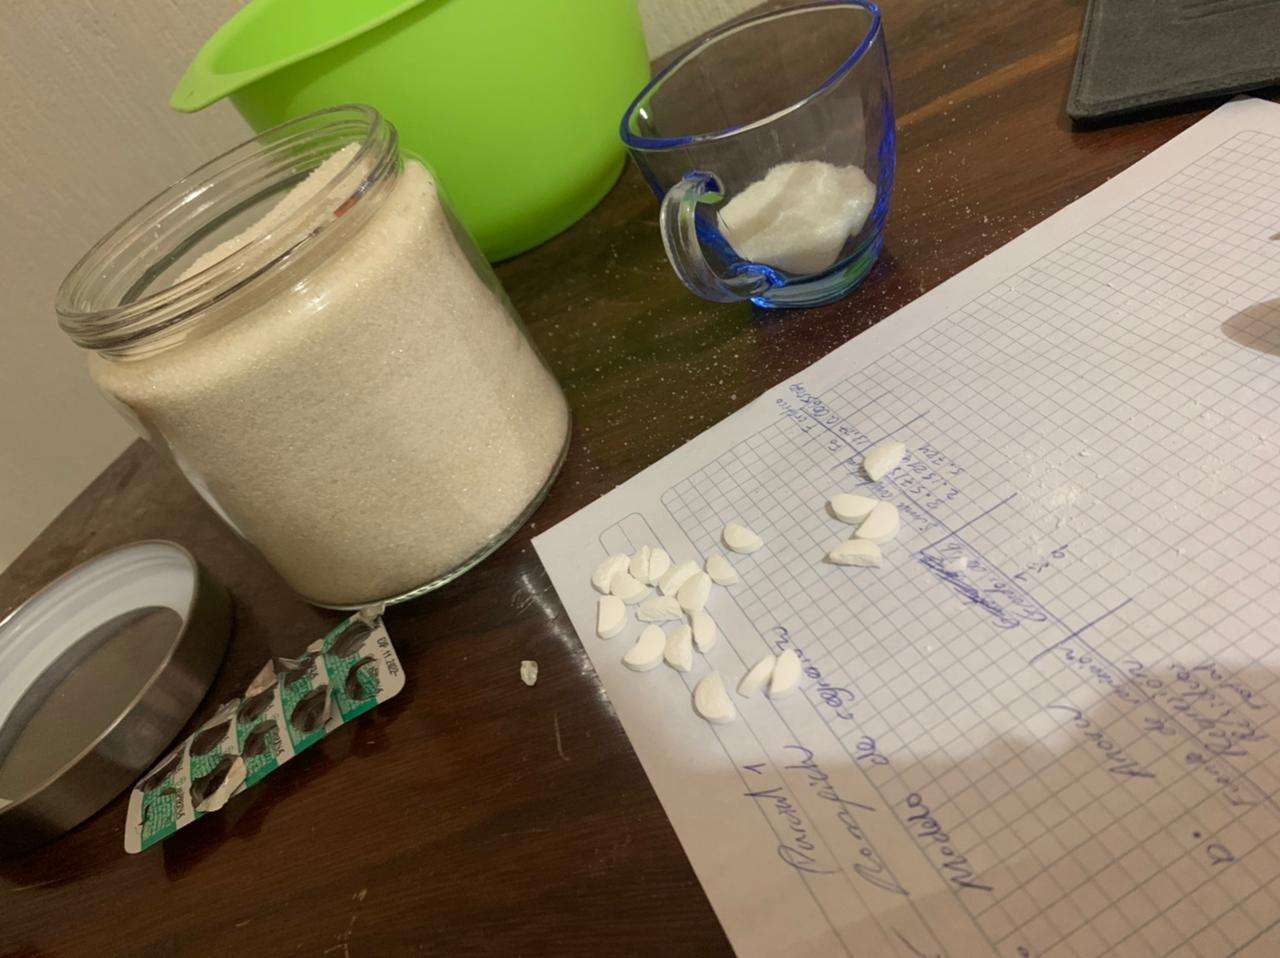
\includegraphics[scale=0.2]{Imagenes/1.JPG}
\end{center}
\begin{center}
    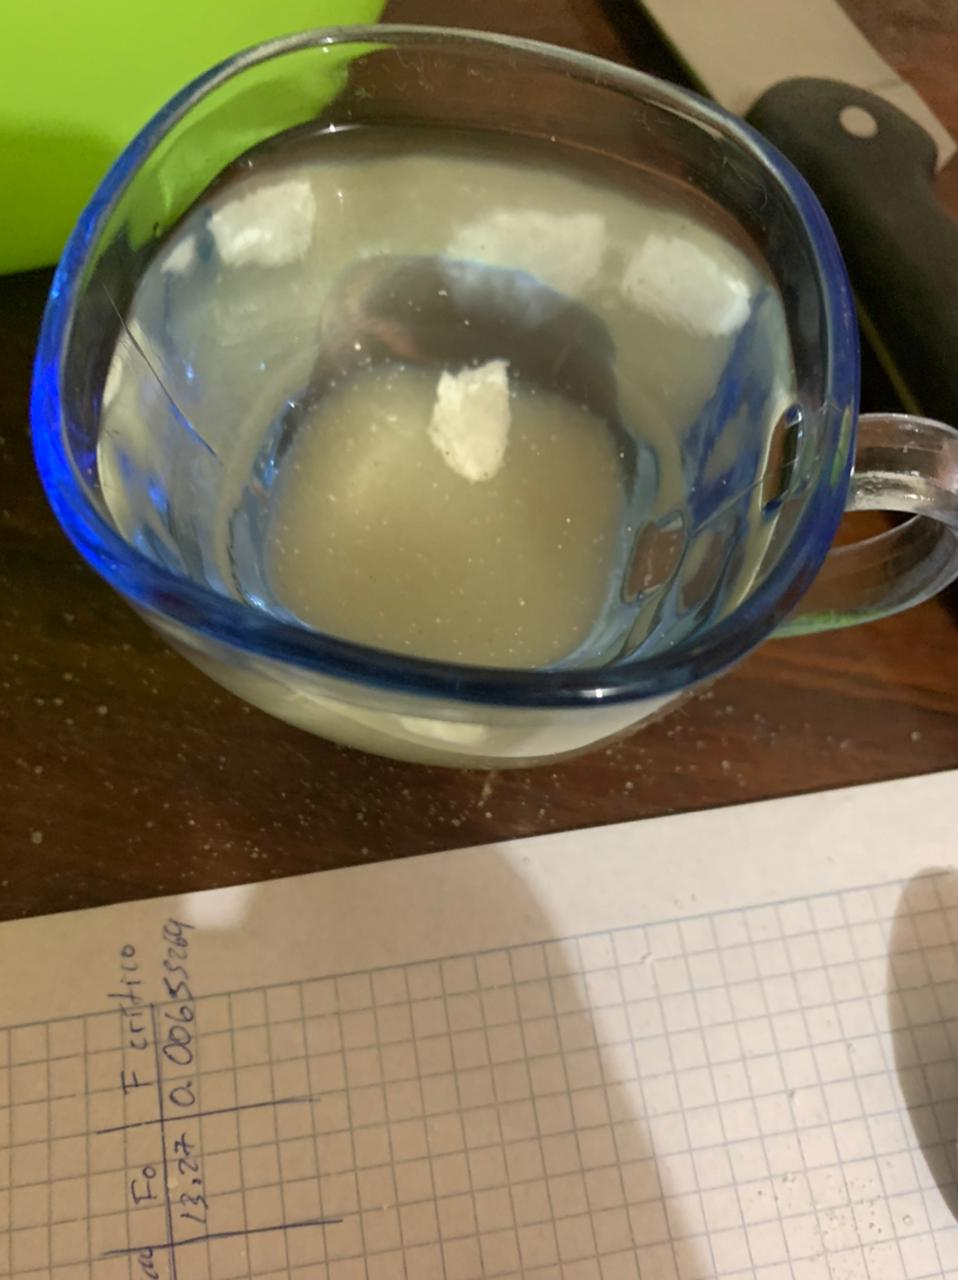
\includegraphics[scale=0.2]{Imagenes/2.JPG}
\end{center}
\begin{center}
    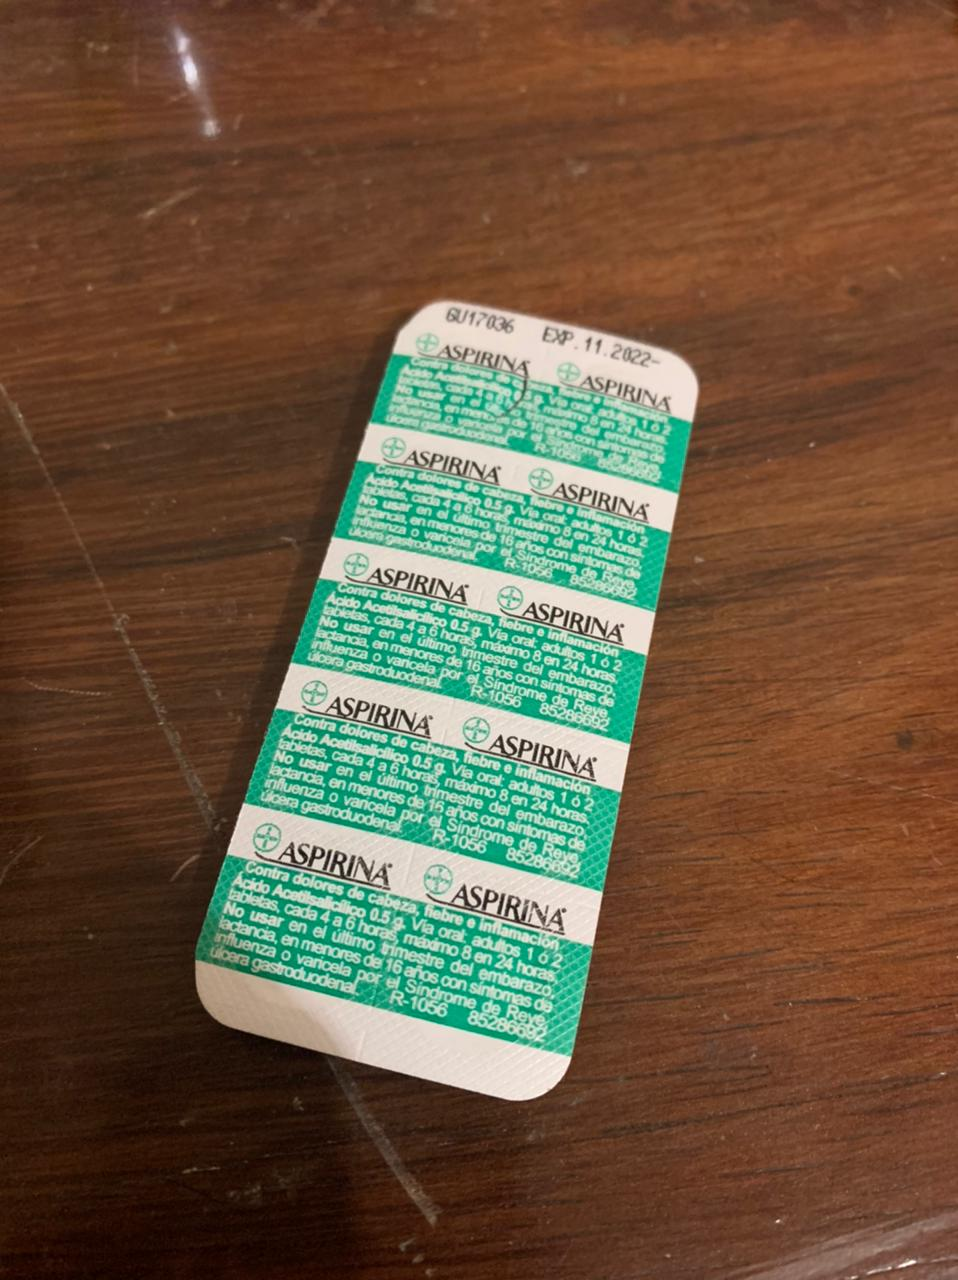
\includegraphics[scale=0.2]{Imagenes/3.JPG}
\end{center}
\begin{center}
    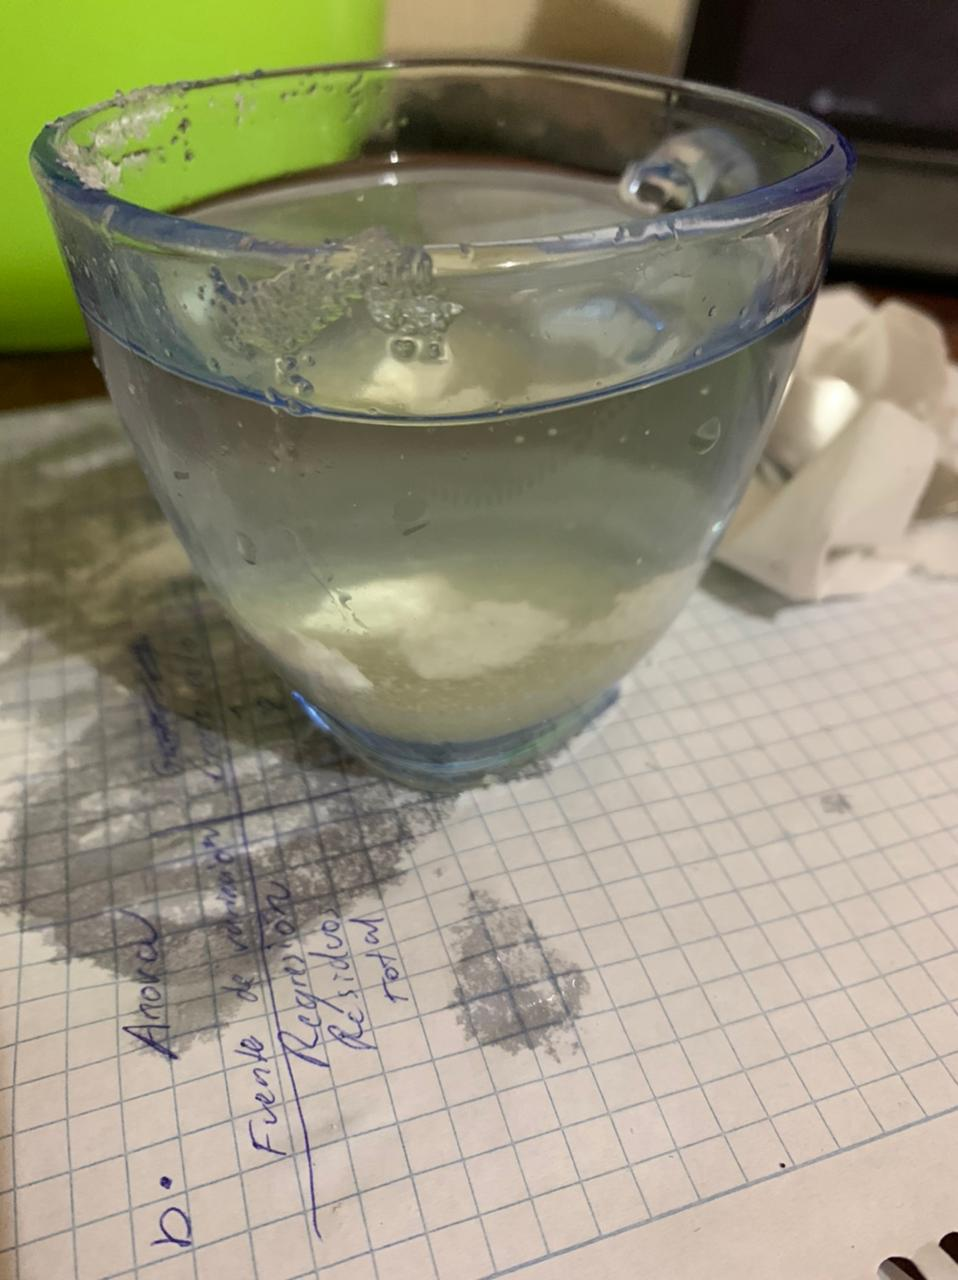
\includegraphics[scale=0.2]{Imagenes/4.JPG}
\end{center}
\begin{center}
    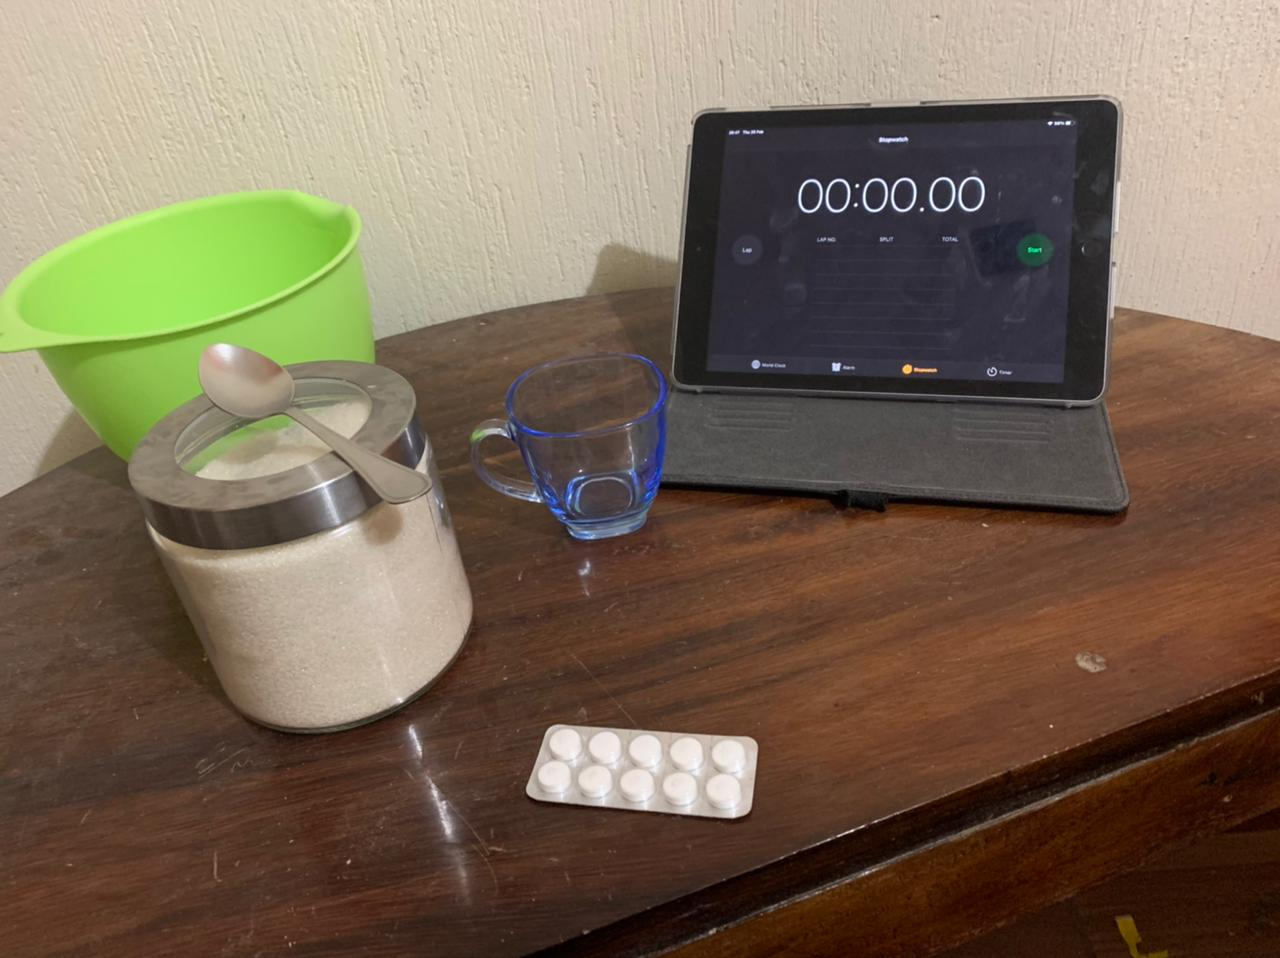
\includegraphics[scale=0.2]{Imagenes/5.JPG}
\end{center}


\subsection{Preguntas}
\begin{enumerate}
    \item ¿cuál es el factor?
    \begin{solution}
    El factor hace referencia a las cucharadas de azúcar disueltas en agua que se usarán en la experimentación. 
    \end{solution}
    \item ¿cuántos niveles tiene el factor?
    \begin{solution}
    Se determinaron 6 niveles para la experimentación en función de las cantidades de azúcar.
    \end{solution}
    \item ¿cuáles son los niveles del factor?
    \begin{solution}
    0.5 cucharadas, 1 cucharada, 1.5 cucharadas, 2 cucharadas, 2.5 cucharadas y 3 cucharadas.
    \end{solution}
    \item ¿cuántas réplicas se harán con cada nivel?
    \begin{solution}
    Por la poca cantidad de aspirinas, solo se trabajarán 4 replicas por cada nivel. 
    \end{solution}
    \item ¿el diseño es de efectos fijos o aleatorios?
    \begin{solution}
    Es fijo, ya que las conclusiones se enfocarán en analizar cada nivel independientemente e individualmente.
    \end{solution}
    \item ¿el diseño es balanceado o no?
    \begin{solution}
    Es balanceado, ya que se tomarán 4 mediciones por cada nivel. 
    \end{solution}
    \item ¿cuál es la variable de respuesta?
    \begin{solution}
    Hace referencia al tiempo que tarda la aspirina en disolverse en el agua con azúcar. Se trabajará en segundos para mayor comodidad.
    \end{solution}
    \item ¿cómo se aleatorizarán las unidades experimentales?
    \begin{solution}
   Por cada nivel, se harán 4 replicas, cada experimento se tratará independientemente, el vaso se llenará con agua y azúcar cada vez que se terminé el anterior experimento; provocando ninguna relación entre los experimentos. 
    \end{solution}
\end{enumerate}
\subsection{Datos experimentales}
Tiempo en segundos.
\begin{center}
    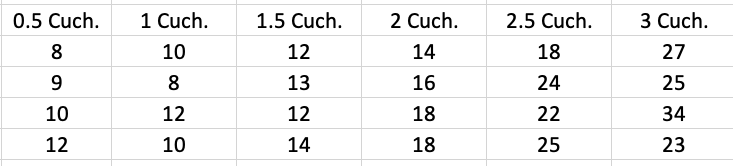
\includegraphics[scale=0.5]{Imagenes/experimentales.png}
\end{center}
\section{Resultados}
\subsection{Pregunta 1}
¿Hay evidencia estadística que apoye la sospecha del directivo de Alfabeta-pharm?
\begin{solution}
   Considerando:
   \begin{center}
       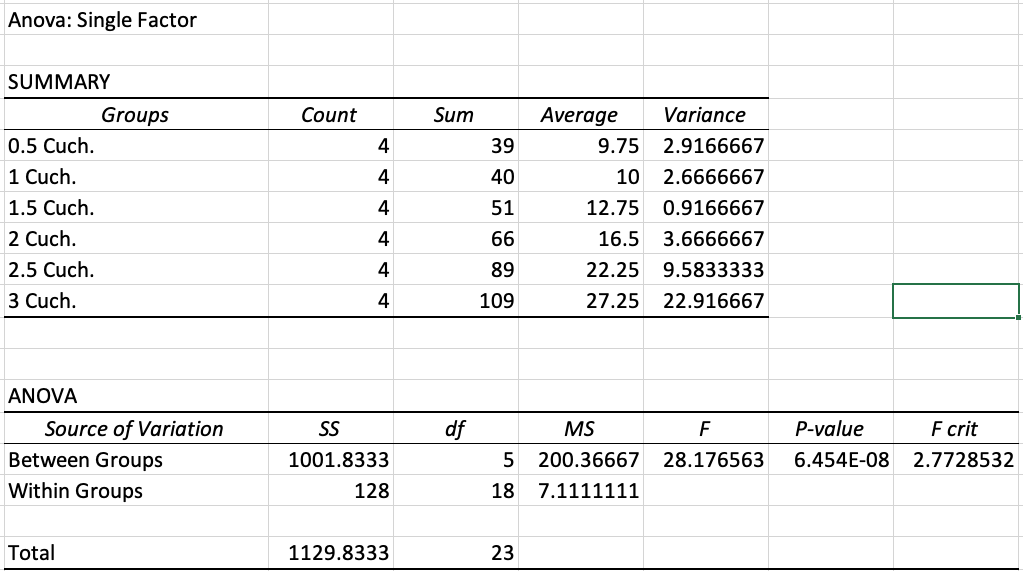
\includegraphics[scale=0.3]{Imagenes/ANOVA.png}
   \end{center}
   Es decir, si usamos la prueba F, quiere decir que el $F$ obtenido es mayor al $F_\alpha$. Es decir que la $H_0$ se rechaza. En otras palabras, se dice que las medias no son iguales y confirmando que la sospecha del directivo de Alfabeta-pharm es correcta. 
\end{solution}

\subsection{Pregunta 2}
Si hay evidencia significativa, ¿Qué niveles de glucosa difieren significativamente entre si?

\begin{solution}
   Analizando los posibles casos, primero analizamos las variables, para aplicar el método de LSD de Fischer:
   \begin{align}
       \intertext{Proponemos un cambio de variables, en donde cada $x_n$ hace referencia a las \textbf{medias aritméticas}:}
       \text{0.5 Cuch.} &= x_1\\
       \text{1 Cuch.}   &= x_2\\
       \text{1.5 Cuch.} &= x_3\\
       \text{2 Cuch.}   &= x_4\\
       \text{2.5 Cuch.} &= x_5\\
       \text{3 Cuch.}   &= x_6
   \end{align}
   Entonces, tenemos los siguientes posibles casos: $|x_1-x_2|, |x_1-x_3|, |x_1-x_4|, |x_1-x_5|, |x_1-x_6|, |x_2-x_3|, |x_2-x_4|, |x_2-x_5|, |x_2-x_6|, |x_3 -x_4|, |x_3 -x_5|, |x_3-x_6|, |x_4-x_5|, |x_4-x_6|, |x_5-x_6|$\newline\newline 
   Asumiendo el LSD de Fischer con un $\alpha=0.05$ de significancia, entonces, tenemos: 
   \begin{center}
       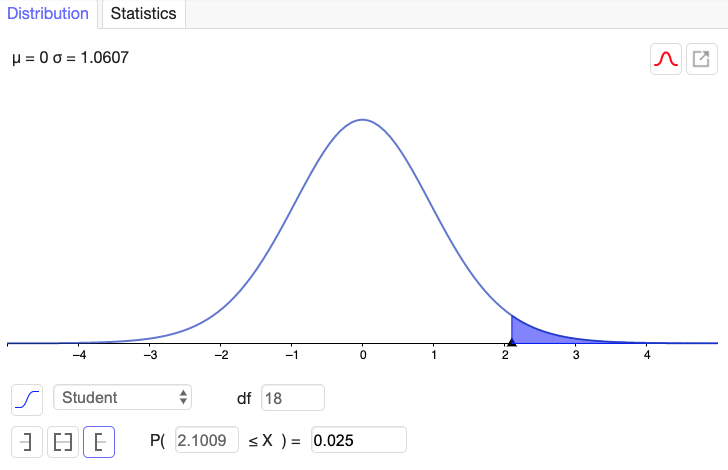
\includegraphics[scale=0.5]{Imagenes/t-student.png}
   \end{center}

Es decir: 
\begin{align}
     LSD &= t_{\alpha/2}\sqrt{CME\left(\frac{1}{n_i}+\frac{1}{n_j}\right)}\\
         &= t_{0.025}\sqrt{7,11111\left(\frac{1}{4}+\frac{1}{4}\right)}\\
         &= (2.1009)\sqrt{7,11111\left(\frac{2}{4}\right)}\\
         &= 3,961
\end{align}
Entonces, aplicando una comparación para cada espacio métrico (distancia): 
\begin{align}
    |x_1-x_2| &= |(9,75)-(10)| &= 0,25\\
    |x_1-x_3| &= |(9,75)-(12,75)| &= 3\\
    |x_1-x_4| &= |(9,75)-(16,5)| &= 6,75\\
    |x_1-x_5| &= |(9,75)-(22,25)| &= 12,75\\
    |x_1-x_6| &= |(9,75)-(27,25)| &= 17,5\\
    |x_2-x_3| &= |(10)-(12,75)| &= 2,75\\
    |x_2-x_4| &= |(10)-(16,5)| &= 6,5\\
    |x_2-x_5| &= |(10)-(22,25)| &=12,25\\
    |x_2-x_6| &= |(10)-(27,25)| &=27,25\\
    |x_3-x_4| &= |(12,75)-(16,5)| &=3,75\\
    |x_3-x_5| &= |(12,75)-(22,25)| &= 9,5\\
    |x_3-x_6| &= |(12,75)-(27,25)| &=14,5\\
    |x_4-x_5| &= |(16,5)-(22,25)| &=5,75\\
    |x_4-x_6| &= |(16,5)-(27,25)| &= 10,75\\
    |x_5-x_6| &= |(22,25)-(27,25)| &=5
\end{align}
Concluyendo que solo (1), (2), (6), (10) son menores a la LSD de Fischer y no existiendo una diferencia significativa, es decir, sus niveles de glucosa no difieren significativamente. Por otra parte, los incisos (3), (4), (5), (7), (8), (9), (11), (12), (13), (14) y (15) sí presentan diferencias significativas ya que no cumplen que $|x_j-x_j|\leq LSD$, es decir, sus niveles de glucosa difieren significativamente.
\end{solution}
\end{document}